\PassOptionsToPackage{unicode=true}{hyperref} % options for packages loaded elsewhere
\PassOptionsToPackage{hyphens}{url}
%
\documentclass[10pt,french,A4]{article}
\usepackage{mathrsfs}
\usepackage{eurosym}
\usepackage{amsmath,amssymb,amsfonts}

\usepackage[T1]{fontenc}
\usepackage[french]{babel}

\usepackage[utf8]{inputenc}
\usepackage{aeguill}
\usepackage{hyperref}
\usepackage{array}
\makeatletter
%%%%%%%%%%%%%%%%%%%%%%%%%%%%%% Textclass specific LaTeX commands.
\usepackage{framed}
\usepackage[framed]{ntheorem}
\newframedtheorem{theoreme}{Théorème}

%definition
\def\theoremframecommand#1{\vrule\hspace{6pt}\hbox{#1}}
\setlength\theorempreskipamount{0pt}%
\setlength\theorempostskipamount{0pt}%
\newshadedtheorem{definition}{\protect\definitionname}
\theoremprework{%
    \setlength\theorempreskipamount{\topsep}%
    \setlength\theorempostskipamount{\topsep}%
}
\theoremstyle{plain}
\theorembodyfont{\upshape}
\newtheorem*{remarque}{Remarque}
\newframedtheorem{propriete}{Propriété}
\newtheorem*{proof}{Preuve}
\newtheorem*{exemple}{Exemple}
\newtheorem{exercice}{Exercice}

% Définition des environnements pour les théorèmes, proposition, etc...

\providecommand{\definitionname}{Définition}
\providecommand{\definitionname}{exemple}
\providecommand{\definitionname}{preuve}
\providecommand{\definitionname}{remarque}
\providecommand{\definitionname}{propriete}
%\providecommand{\theoremname}{Théorème}
%%%%%%%%%%%%%%%%%%%%%%%%%%%%%% User specified LaTeX commands.

\usepackage{fourier} % math & rm
\usepackage[scaled=0.875]{helvet} % ss
\usepackage[normalem]{ulem}
\usepackage{pifont}
\usepackage[tikz]{bclogo}
\usetikzlibrary{positioning,shapes,decorations}
\usepackage{wrapfig}
\usepackage{mathrsfs}
\usetikzlibrary{arrows}
\usepackage{multicol}

\setlength{\columnseprule}{0.5pt}
\setlength{\columnsep}{20pt}
\usepackage{smartdiagram}
\usepackage[paperwidth=210mm,paperheight=297mm]{geometry}
\geometry{verbose,tmargin=2cm,bmargin=15mm,lmargin=2cm,rmargin=2cm,headheight=1cm,headsep=5mm,footskip=5mm}
\usepackage{fancyhdr}
\usepackage{hyperref}
\hypersetup{
            pdftitle={Les Signaux},
            pdfauthor={Pascal Malingrey},
            pdfkeywords={NSI, Signaux, Linux},
            pdfborder={0 0 0},
            pdfsubject={Les signaux sur Linux},
            breaklinks=true}
\urlstyle{same}  % don't use monospace font for urls
\usepackage{xcolor}
\usepackage[tikz]{bclogo}
\usepackage{wrapfig}
\usepackage{framed}
\usepackage{algorithm}
\usepackage{algpseudocode}%MISE EN PAGE

\usepackage{listings,lipsum,listingsutf8}
\definecolor{codegreen}{rgb}{0.1,0.47,0.1}
\definecolor{fondjaune}{rgb}{0.99, 0.7,0.8}
\definecolor{couleurdef}{rgb}{0.99, 0.8, 0.87}
\definecolor{codegray}{rgb}{0.5,0.5,0.5}
\definecolor{codepurple}{rgb}{0.58,0,0.82}
\definecolor{backcolour}{rgb}{0.95,0.95,0.92}

\newenvironment{code}[1]{%
    \begin{bclogo}[couleur=backcolour, couleurTexte=black ,couleurBord=blue ,couleurBarre=black, ombre=false,epBord=0.9,logo=\#,arrondi=0.1]{{\bfseries #1}}%
    }%
    {%
    \end{bclogo}
}%
%---------------------------- version élève - prof
\newboolean{Prof}

\newcommand{\cacher}[1]{
    \ifthenelse{\boolean{Prof}} % si « Professeur » est vrai,
    {#1} %les mots cachés sont en gras
    {\dashuline{\phantom{#1}}} % (else) sinon les mots sont remplacés par une ligne sur laquelle l'élève peut écrire. 
}
\newcommand{\cacherb}[1]{
    \ifthenelse{\boolean{Prof}} % si « Professeur » est vrai,
    {#1} %les mots cachés sont en gras
    {\phantom{#1}} % (else) sinon les mots sont remplacés par une ligne sur laquelle l'élève peut écrire. 
}
%-------------------------------------------------------
\usepackage{minted}
\title{Les Signaux}
\author{Pascal Malingrey}
\date{}
%------------------------------------------------------------
\usepackage{fancyhdr}
\pagestyle{fancy}
\chead{\Large Les Signaux}
\lfoot{\scriptsize P.MALINGREY}
\rhead{DIU: Bloc3}
\begin{document}
\setboolean{Prof}{true}  %----------------version prof

  \ifProf
\section*{Prérequis}
\begin{enumerate}
    \item Système d'exploitation : Linux
    \item Les notions de base sur le fonctionnement du noyau et les processus.
    \item Utilisation du  terminal (shell)
    \item Python: 
    \begin{itemize}
        \item écriture d'une fonction
        \item avoir vu \textit{try except} est un plus (gestion des erreurs avec Python)
    \end{itemize}
\end{enumerate}
\section*{Organisation}
\begin{itemize}
\item La séance est prévue pour être faite une partie en classe entière ou idéalement en salle informatique et la séance d'exercices en salle informatique. (1h+1h). 
\item matériels: poste sous Linux avec Python3 installé.
\item La  feuille de cours est à compléter (il s'agit de la partie les notions).
\item Un diaporama accompagne les fiches afin d'apporter des précisions sur les notions abordées.
\end{itemize}
\section*{Compétences visées}
\begin{itemize}
    \item Comprendre comment  les processus échangent des informations entre eux à l'aide des signaux.
    \item Utilisation de la commande kill.
    \item Implémentation des signaux avec Python, écriture des gestionnaires de signaux.
\end{itemize}

\tableofcontents

\newpage
\fi

\section{Première approche}


\subsection{STOP ou ENCORE}
Vous disposez dans votre dossier d'un fichier \textbf{ex1.py} (son contenu n'a pas d'importance pour le moment.)
Dans un terminal vous exécuter la commande suivante:
\begin{code}{terminal}
\begin{minted}{bash}
nsi@lin$ python3 ex1.py
\end{minted}
\end{code}

\begin{enumerate}
\item Que constatez vous ?
\item Comment interrompre le programme , tout en gardant le terminal actif?

 \cacher{On va appuyer sur une combinaison de touche \texttt{Ctrl+C}}
\end{enumerate}

\subsection{Que s'est-il passé?}

La combinaison de touche \cacher{\texttt{Ctrl+C}} a interrompu l' exécution du programme.
Cela signifie deux choses:

\begin{itemize}
\item \cacher{ ``quelque chose'' est à l'écoute du clavier}
\item \cacher{ un programme traite l'information de la combinaison \texttt{Ctrl+C}}
\end{itemize}

\hypertarget{deuxiuxe8me-approche}{%
\section{Deuxième approche}\label{deuxiuxe8me-approche}}
\begin{multicols}{2}
    \hypertarget{commande-shell}{%
        \subsection{Commande shell}\label{commande-shell}}
    
    La commande \texttt{cat} est utilisée qu'à titre d'exemple, sa
    fonctionnalité n'est pas importante ici. Par contre les suivantes sont
    utiles:
    
    \begin{itemize}
        \item \texttt{ps} : liste les processus dans le terminal
        \item \texttt{\^{}z} : Ctrl+z suspend un processus
        \item \texttt{fg} : reprend un processus
    \end{itemize}

\subsection{Dans un terminal}
\begin{enumerate}   
    \item  Liste des commandes : \textit{à taper}
        \begin{code}{terminal}
            \begin{minted}{bash}
nsi@lin$ cat
nsi@lin$ ^z  # Appui sur Ctrl+z
nsi@lin$ ps
            \end{minted}
        \end{code}
        \item résultat : \textit{à compléter}
  \ifProf
 \begin{code}{terminal}
        \begin{minted}{bash}
PID TTY          TIME CMD
25280 pts/0    00:00:00 bash
26623 pts/0    00:00:00 cat
26624 pts/0    00:00:00 ps
        \end{minted}
\end{code}
  \else
     \begin{code}{terminal}
        \begin{minted}{bash}
PID TTY          TIME CMD
.
.
.
\end{minted}
\end{code}
\fi

        \item{Stoppons le processus cat}
             \begin{itemize}
        \item
        Nous allons envoyer un signal de terminaison au processus cat par le biais de la commande \textbf{killall} qui envoie un signal aux processus dont le nom est indiqué avec le numéro du signal. 
        \begin{code}{terminal}
            \begin{minted}{bash}
nsi@lin$ killall -2 cat
            \end{minted}
        \end{code}
        \item Regardons ce qui s'est passé
        \begin{code}{terminal}
            \begin{minted}{bash}
nsi@lin$ ps
            \end{minted}
        \end{code}
        \item  Que remarque-t-on? \vskip 0.5cm
        \cacherb{Le processus \texttt{cat} est toujours présent. En fait il a été
        suspendu par la commande \texttt{\^{}z}.}
        \item On va demander une reprise du processus avec la commande \texttt{fg}
        \begin{code}{terminal}
            \begin{minted}{bash}
nsi@lin$ fg
nsi@lin$ ps
            \end{minted}
        \end{code}
        \item Que remarque-t-on? \vskip 0.5cm
 \end{itemize}

\end{enumerate}
\end{multicols}

\subsection{Conclusion}
   Suite à la reprise du processus, le signal  \cacher{\textbf{Ctrl-C }}  a été exécuté.   Le signal d'interruption n'est traité que lorsque le processus
    \texttt{cat} redevient actif, c'est donc bien le processus qui traite
    l'information du signal \textbf{  2 }, dont il est destinataire. Cela signifie également que le signal\textbf{ 2 }a été
    mémorisé par le système. 
    
\noindent
\begin{tikzpicture}
[node distance = 1cm, auto,
nodes={draw, ultra thick, fill=blue!20},
every node/.style={node distance=3cm},
% The comment style is used to describe the characteristics of each force
comment/.style={rectangle, inner sep= 2pt, text width=2cm, node distance=0.25cm, font=\scriptsize\sffamily},
% The force style is used to draw the forces' name
force/.style={rectangle, draw, fill=black!8, inner sep=2pt, text width=2cm, text badly centered, minimum height=1.2cm, font=\bfseries\footnotesize\sffamily}
] 
% Draw forces
\draw[->](0,0)node[force]{processus cat:\\ lancé}--++(4,0)node[force]{processus cat:\\ \cacher{stoppé}}--++(4,0)node[force]{processus cat:\\ \cacher{tjs stoppé}}--++(4,0)node[force]{processus cat:\\ \cacher{reprise}}--++(4,0)node[force]{processus cat:\\ \cacher{tué}};
\draw(2.8,-0.3)node[comment]{Ctrl-Z};
\draw(6.5,-0.3)node[comment]{killall -2 cat};
\draw(11,-0.3)node[comment]{fg};
\draw(14.2,-0.3)node[comment]{Action de killall};
\end{tikzpicture}
\ifProf
\textit{En fait les choses sont un peu plus compliquées : cf annexe }
\fi
\begin{bclogo}[couleur=couleurdef, couleurTexte=black ,couleurBord=black ,couleurBarre=blue, ombre=false,epBord=0.9,logo=\bcbook,arrondi=0.1]{{\bfseries Commande }}
    \begin{itemize}
        \item[\textbullet] {\bfseries ps :} liste les processus actifs attachés au terminal, les processus sont identifiés par leur PID.
        \item[\textbullet] {\bfseries kill :} commande permettant d'envoyer  un signal à un processus identifié par son PID avec le numéro du signal. 
        \item[\textbullet] {\bfseries killall :} commande permettant d'envoyer  un signal \underline{aux} processus dont le nom est indiqué avec le numéro du signal. 
    \end{itemize}
\end{bclogo}

\hypertarget{les-notions}{%
\section{Les notions}\label{les-notions}}

\hypertarget{duxe9finition-dun-signal}{%
\subsection{Définition d'un signal}\label{duxe9finition-dun-signal}}

\begin{definition}
Un signal est :
\begin{itemize}
\item un message envoyé par le noyau de manière \emph{asynchrone} à :
  \begin{itemize}
  \item un processus ; ou
  \item  un groupe de processus
  \end{itemize}
\item pour indiquer un événement système important
\end{itemize}
\end{definition}
 Le message peut être à l'initiative d'un autre processus.
Cette communication limitée \textbf{(seul le numéro du signal est envoyé) } entre
les processus. La norme POSIX définit un certain nombre de signaux, environ une vingtaine.  (voir 3.3) 

\hypertarget{schuxe9ma-1}{%
\subsection{Schéma 1}\label{schuxe9ma-1}}
\begin{tikzpicture}
[node distance = 1cm, auto,
nodes={draw, ultra thick, fill=blue!20},
every node/.style={node distance=3cm},
% The comment style is used to describe the characteristics of each force
comment/.style={rectangle, inner sep= 5pt, text width=3cm, node distance=0.25cm, font=\scriptsize\sffamily},
% The force style is used to draw the forces' name
force/.style={rectangle, draw, fill=black!8, inner sep=5pt, text width=3cm, text badly centered, minimum height=1.2cm, font=\bfseries\footnotesize\sffamily}
] 
% Draw forces
\node [circle,draw, minimum height=1.5cm,thick, fill=blue!20] (noyau) {Noyau};

\node [force, right =3cm of  noyau] (processus) {Processus\\ex: cat};
\node [force, text width=3cm, dashed, left=3cm of noyau] (evt) {événement\\
    ex: Ctrl-C};
\draw[->](evt)--(noyau)node[above, midway]{capté par le noyau};
\draw[->](noyau)--(processus)node[midway, above]{signal};
\end{tikzpicture}

Quelques événements possibles
\begin{itemize}
    \item frappe de caractère dans un terminal \textit{(c'est interpréteur de commande qui envoie  un signal)}
    \begin{itemize}
        \item  \texttt{Ctrl+C} 
        \item \texttt{Ctrl+Z} etc.
    \end{itemize}
    \item terminaison d'un processus
    \item un problème matériel : division par zéro, problème d'adressage, défaillance d'alimentation électrique, etc.
    \item l'expiration de délai préprogrammé (fonction alarm())
    \item ...
\end{itemize}

\hypertarget{}{%
\subsection{Les différents signaux}\label{schuxe9ma-2}}
Exécuter la commande ci-dessous pour avoir la liste des signaux disponibles
\begin{code}{terminal}
    \begin{minted}{bash}
nsi@lin$ kill -l
    \end{minted}
\end{code}

La norme POSIX distingue  32 signaux dont les principaux sont: \textit{compléter le tableau}
\begin{center}

\begin{tabular}{|c|c|c|c|}
    \hline 
Numéro & Nom & Signification & Comportement\\ 
    \hline 
1&SIGHUP & Hang-up (fin de connexion) & T(erminaison)\\ 
    \hline 
 2 &  \cacherb{SIGINT} &Interruption (Ctrl-C)  &T\\ 
    \hline 
\cacherb{3}    &SIGQUIT & Interruption forte (Ctrl-$\backslash$) & T + core\\ 
    \hline 
 \cacherb{8}   &SIGFPE & Erreur arithmétique & T + core\\ 
    \hline 
    9 &\cacherb{SIGKILL} & Interruption immédiate et absolue & T + core\\ 
    \hline 
\cacherb{11}   &SIGSEGV&Violation des protections mémoire &T + core\\ 
    \hline 
 \cacherb{13}   &SIGPIPE &Écriture sur un pipe sans lecteurs& T\\ 
    \hline 
   20 & \cacherb{SIGTSTP} &Arrêt temporaire(Ctrl-Z)& Suspension\\ 
    \hline 
   18 &SIGCONT& Redémarrage d’un fils arrêté & Ignoré \\ 
    \hline 
 \cacherb{17}     &SIGCHLD &un des fils est mort ou arrêté & Ignoré \\ 
    \hline 
    14 &\cacherb{SIGALRM} & Interruption d'horloge & Ignoré \\ 
    \hline 
   19 &\cacherb{SIGSTOP} & Arrêt temporaire & Suspension \\ 
    \hline 
  \cacherb{10}    &SIGUSR1 & Émis par un processus utilisateur & T \\ 
    \hline 
 \cacherb{12}     &SIGUSR2 & Émis par un processus utilisateur & T \\ 
    \hline 
\end{tabular} 
\end{center}
T: terminaison du processus
; core: création d'un fichier d'image mémoire

\begin{remarque}
    Quelle différence entre SIGSTP et SIGSTOP, de même entre SIGINT et SIGKILL?\\
    \cacherb{
    Certains signaux ne peuvent être bloqués ou ignorés par le processus, c'est le cas de de SIGSTOP et SIGKILL.
    SIGINT laisse la possibilité au processus d'ignorer et/ou de contrôler le signal par contre avec SIGKILL aucun moyen de passer outre la demande d'interruption.
    De même pour SIGSTOP, le signal ne peut pas être ignoré et modifié.\\ 
    Pour la liste de toutes les actions des signaux:
    \url{http://www.linux-france.org/article/man-fr/man7/signal-7.html}}
\end{remarque}

\begin{exemple}
    Reprenons l'approche 2. Indiquez le nom (dans la nomemclature POSIX ) des signaux envoyés et les actions entre chacune des phases.
    
    \hskip -0.5cm\begin{tikzpicture}
    [node distance = 1cm, auto,
    nodes={draw, ultra thick, fill=blue!20},
    every node/.style={node distance=3cm},
    % The comment style is used to describe the characteristics of each force
    comment/.style={rectangle, inner sep= 2pt, text width=2cm, node distance=0.25cm, font=\scriptsize\sffamily},
    % The force style is used to draw the forces' name
    force/.style={rectangle, draw, fill=black!8, inner sep=2pt, text width=2cm, text badly centered, minimum height=1.2cm, font=\bfseries\footnotesize\sffamily}
    ] 
    % Draw forces
    \draw[->](0,0)node[force]{processus cat:\\lancé}--++(4,0)node[force]{processus cat:\\stoppé}--++(4,0)node[force]{processus cat:\\tjs stoppé}--++(4,0)node[force]{processus cat:\\reprise}--++(4,0)node[force]{processus:\\tué};
    \draw(2.8,-0.3)node[comment]{\cacher{SIGSTP}\\ \cacherb{suspension}};
    \draw(6.5,-0.3)node[comment]{\cacher{SIGINT}\\ \cacherb{aucun}};
    \draw(10.7,-0.3)node[comment]{\cacher{SIGCONT}\\ \cacherb{ignoré}};
    \draw(14.4,-0.3)node[comment]{\cacher{...}\\ \cacherb{terminaison}};
    \end{tikzpicture}
\end{exemple}
\hypertarget{que-se-passe-t-il-uxe0-la-ruxe9ception-du-signal}{%
\subsection{Que se passe-t-il à la réception du signal
?}\label{que-se-passe-t-il-uxe0-la-ruxe9ception-du-signal}}

\begin{itemize}
\item
  Terminaison de l'exécution.
\item
  Suspension de l'exécution (le processus père est prévenu).
\item
  Rien : le signal est ignoré.
\item
  Exécution d'une fonction définie par l'utilisateur.
\end{itemize}

\hypertarget{gestion-des-signaux}{%
\subsection{Résumé et un peu plus : Gestion des signaux}\label{gestion-des-signaux}}

La prise en compte d'un signal (on parle de \textbf{délivrance}) ne peut avoir
lieu que dans une circonstance bien particulière : la bascule du mode
noyau au mode utilisateur. Lorsqu'un signal est envoyé à un processus,
plusieurs cas peuvent se produire :
 
 \begin{tikzpicture}
[node distance = 1cm, auto,
nodes={draw, ultra thick, fill=blue!20},
every node/.style={node distance=3cm},
% The comment style is used to describe the characteristics of each force
comment/.style={rectangle, inner sep= 5pt, text width=3cm, node distance=0.25cm, font=\scriptsize\sffamily},
% The force style is used to draw the forces' name
force/.style={rectangle, draw, fill=black!8, inner sep=5pt, text width=2cm, text badly centered, minimum height=1cm, font=\bfseries\footnotesize\sffamily}
] 
% Draw forces
\draw(-0.3,-1.8)node[force]{processsus 2};
\draw(5,0.5)node[force]{processus 2};
\draw(10,0.5)node[force]{processus 2};
\draw(-3.5,0)node{mode utilisateur};
\draw(-3.5,-1.5)node{mode noyau};
\draw[dashed](-3,-1)--(12,-1);
\draw[thin,->](2.5,1)--(2.5,-2)node[comment,below]{fin du quota de temps};
\draw[thin,->](7.5,1)--(7.5,-2)node[comment,below]{ou  retour d'un appel système};
\draw[->](3,-1.5) to[bend left,thick] (3.2,-0.5);
\draw[->](8,-1.5) to[bend left,thick]  (8.2,-0.5);
%\draw(-2,-1) -- (2.5,-1);
\draw(5,-0.5)node[comment]{actions sur les signaux};
\draw(10,-0.5)node[comment]{actions sur les signaux};
\end{tikzpicture}

\begin{itemize}
\item
  Le processus est en mode utilisateur :\\
  La délivrance devra alors
  attendre d'abord le passage du processus en mode noyau puis son
  retour au mode utilisateur. Pendant tout ce temps, le signal sera
  \textbf{pendant}, c'est à dire en attente de \textbf{délivrance}.
\item
  Le processus est en mode noyau, par définition non interruptible. Le
  signal sera délivré dès que le processus reviendra au mode
  utilisateur: le signal est donc \textbf{pendant}. Lorsque le signal est délivré, la procédure qui lui
  est associée (son gestionnaire ou\textbf{ handler})  est appelée. L'action du signal peut être:
  \begin{enumerate}
      \item  le comportement par défaut (par exemple l'interruption)
      \item l'ignorance
      \item le traitement personnalisé
      \item le masquage (blocage)
  \end{enumerate}
\begin{center}
    \textbf{Le gestionnaire ou handler}
\end{center}


 \begin{tikzpicture}
[node distance = 1cm, auto,
nodes={draw, ultra thick, fill=blue!20},
every node/.style={node distance=3cm},
% The comment style is used to describe the characteristics of each force
comment/.style={rectangle, inner sep= 5pt, text width=3cm, node distance=0.25cm, font=\scriptsize\sffamily},
% The force style is used to draw the forces' name
force/.style={rectangle, draw, fill=black!8, inner sep=5pt, text width=3.5cm, text badly centered, minimum height=1cm, font=\bfseries\footnotesize\sffamily}
] 
\draw[-latex,very thick](0,0)node[left]{processsus}--(1.9,0); \draw[-latex,very thick]((2.1,0)--(6,0);
\draw[-latex,color=red!60!black,decorate,decoration=zigzag](2,2)node[above]{signal}--(2,0.1);
\draw[-latex,blue](2,-0.1)--(2,-1)--(4,-1)node[comment,midway,below]{Exécution du gestionnaire};
\draw[-latex,blue](4,-1)to[bend left=-90, out = -90](2.1,0); \draw(4.5,1)node[force]{Le gestionnaire retourne à l'endroit où l'exécution a été interrompue};
\end{tikzpicture}
 \begin{tikzpicture}
[node distance = 1cm, auto,
nodes={draw, ultra thick, fill=blue!20},
every node/.style={node distance=3cm},
% The comment style is used to describe the characteristics of each force
comment/.style={rectangle, inner sep= 5pt, text width=3cm, node distance=0.25cm, font=\scriptsize\sffamily},
% The force style is used to draw the forces' name
force/.style={rectangle, draw, fill=black!8, inner sep=5pt, text width=3.5cm, text badly centered, minimum height=1cm, font=\bfseries\footnotesize\sffamily}
] 
\draw[-latex,very thick](0,0)node[left]{processsus}--(1.9,0); \draw[-latex,very thick]((2.1,0)--(6,0);
\draw[-latex,color=red!60!black,decorate,decoration=zigzag](2,2)node[above]{signal}--(2,0.1);
\draw[-latex,blue](2,-0.1)--(2,-1)--(4,-1)node[comment,midway,below]{Exécution du gestionnaire};
\draw[-latex,blue](4,-1)to[bend left=-90, out = 90](6,0); \draw(4.5,1)node[force]{Le gestionnaire met fin au processus};
\end{tikzpicture}
 \begin{tikzpicture}
[node distance = 1cm, auto,
nodes={draw, ultra thick, fill=blue!20},
every node/.style={node distance=3cm},
% The comment style is used to describe the characteristics of each force
comment/.style={rectangle, inner sep= 5pt, text width=3cm, node distance=0.25cm, font=\scriptsize\sffamily},
% The force style is used to draw the forces' name
force/.style={rectangle, draw, fill=black!8, inner sep=5pt, text width=3.5cm, text badly centered, minimum height=1cm, font=\bfseries\footnotesize\sffamily}
] 
\draw[-latex,very thick](0,0)node[left]{processsus}--(1.9,0); \draw[-latex,very thick]((2.1,0)--(6,0);
\draw[-latex,color=red!60!black,decorate,decoration=zigzag](2,2)node[above]{signal}--(2,0.1);
\draw[-latex,blue](2,-0.1)--(2,-1)--(4,-1)node[comment,midway,below]{Exécution du gestionnaire};
\draw[-latex,blue](4,-1)to[bend left=90, out =- 90](0.5,0); \draw(4.5,1)node[force]{Le gestionnaire retourne vers un point de reprise sauvegardé antérieurement};
\end{tikzpicture}

Attention: Le signal SIGCONT ne peut être pris en charge par un \textbf{gestionnaire} car il s'adresse à un processus qui est en endormi (SIGSTOP).
\item
  Le signal peut être \textbf{bloqué} (on dit également \textbf{masqué}). Ceci signifie
  que la délivrance du signal est différée jusqu'à ce que le blocage
  soit levé. Ceci n'est possible que pour certains signaux. \\ Lorsqu'un signal bloqué arrive sur le processus, il n'est
  pas supprimé, il est juste mis en attente : il devient donc pendant.
\end{itemize}
\begin{definition}
    Donc les différents états d'un signal sont:
    \begin{description}
        \item[généré/émis:] L'événement associé au signal s'est produit
        \item[délivré:] L'action associée au signal a été exécutée
         \item[pendant:]  Le signal émis n'a pas encore été pris en compte
        \item[bloqué/masqué:] La prise en compte du signal est volontairement différée.
    \end{description}
\end{definition}

L'ensemble des informations des signaux pour un processus est regroupé en un vecteur (un pour chaque processus) indexé sur les numéros de signaux et dont chaque case
comporte 3 informations :

\begin{itemize}
\item
  Un \textbf{booléen} indiquant si le signal est pendant.Cette
  information est un booléen unique. Ce qui signifie que si un processus
  a déjà un signal d'un certain type pendant, il est inutile de lui
  envoyer à nouveau un signal du même type, celui-ci sera ignoré.
\item
  Un\textbf{ booléen} indiquant si les signaux de ce type sont bloqués.
\item
  Un \textbf{pointeur} désignant le gestionnaire (handler).
\end{itemize}

\subsection{Description détaillée des signaux}
\hypertarget{liste-signaux}{ Voir la deuxième  page de l'annexe}

\newpage

\hypertarget{retour-uxe0-la-programmation}{%
\section{Retour à la
programmation}\label{retour-uxe0-la-programmation}}

Nous avons vu dans la première partie que certains signaux peuvent être interceptés par le processus. 

Regardons comment faire à l'aide de Python
\begin{bclogo}[couleur=couleurdef, couleurTexte=black ,couleurBord=black ,couleurBarre=blue, ombre=false,epBord=0.9,logo=\bcbook,arrondi=0.1]{{\bfseries Les signaux avec Python}}
    \begin{itemize}
        \item[\textbullet] {\bfseries signal :} la librairie  \texttt{signal} permet de travailler avec les signaux qui peuvent être modifiés (SIGINT, SIGTERM, SIGSTP, SIGALRM...)
        \item[\textbullet] {\bfseries signal.signal(monsignal, mafonction) :} permet d'exécuter la fonction \textbf{mafonction}, lors de l'apparition du signal \textbf{monsignal}. Il s'agit du gestionnaire (handler) du signal.
        \item[\textbullet] {\bfseries signal.alarm(t) :} envoi un signal alarm après un délai de $t$ secondes.
       \item[\textbullet] {\bfseries signal.SIG... :} permet de faire référence au signal SIG...  (en fait on récupère le numéro du signal).\\
       par exemple signal.SIGTERM fait réféfence au Ctrl-C.
    \end{itemize}
\end{bclogo}
\vskip 1em
\begin{exercice}
 Reprenez le fichier \textbf{ex1.py} et le modifier pour que le signal SIGINT(Ctrl-C) ne puisse pas interrompre le programme.\\
 Quelle commande permet de mettre fin au programme ?
\end{exercice}
\ifProf
\begin{code}{ex1b.py}
\begin{minted}{Python}
import signal, time

def mongestionnaire(signum,stack):
    print("Ctrl-C est désactivé")

signal.signal(signal.SIGINT, mongestionnaire)

i = 1
while 1:
    print("itération :{}".format(i))
    time.sleep(1)
    i += 1
\end{minted}
\end{code}

La commande \textbf{kill -2 pid}(SIGINT)  ne permet plus d'arrêter le programme, il faut donc envoyer un signal d'interruption qui ne peut pas être intercepté ou modifi', il s'agit \textbf{kill - 9 pid} (SIGKILL).
\fi
\vskip 0.5 cm

\begin{exercice}
    Voici un programme:
        \begin{minted}[autogobble, linenos,fontsize=\small]{Python}
    import signal, time
    
    def mongestionnaire(signum, stack):
        print('Alarme :', time.ctime())
       
    signal.signal(signal.SIGALRM, mongestionnaire)
    signal.alarm(2)
    
    print('Première:', time.ctime())
    time.sleep(4)
    print('Terminale :', time.ctime())
   \end{minted}
   
   \begin{enumerate}
       \item Expliquer les commandes des lignes 6 et 7.
       
       \ifProf
    \textbf{Ligne 6: on associe au signal SIGALRM, la fonction mongestionnaire comme handler.}\\
    \textbf{Ligne 7: on envoie le signal SIGALRM au processus actuel avant un temps de 2 secondes d'attente.}
       \fi
       \item Que va afficher le programme, si l'heure de début est 12:00:00 (12h )?
              \ifProf
              
       \textbf{Première : 12:00:00}\\
       \textbf{Alarme : 12:00:02}\\
        \textbf{Terminale : 12:00:02}\\
       \fi
   \end{enumerate}
\end{exercice}

\begin{exercice}
   Notre programme possède une fonction \textbf{inconnue} qui peut prendre beaucoup de temps. Nous aimerions qu'au bout de 5s, celle-ci soit automatiquement interrompue.
   \begin{code}{La fonction inconnue}
        \begin{minted}[autogobble]{Python}
 def inconnue(n):
       while n>0:
           print('je travaille encore  ',n)
           time.sleep(1)
           n -= 1
       \end{minted}
   \end{code}
Apporter les modifications nécessaires, pour réaliser ce que l'on souhaite.
\end{exercice}

\ifProf
\begin{code}{ex3.py}
    \inputminted[fontsize=\small]{Python}{ex3.py}
\end{code}
\fi
\begin{exercice}
    Un programme attend une réponse de l'utilisateur suite à une commande \textbf{input}. On aimerait qu'au bout de 5 secondes un message s'affiche, pour demander de répondre dans les 5 prochaines secondes et si tel n'est pas le cas le programme s'interrompt.
    
\end{exercice}
\ifProf
\begin{code}{ex4.py}
    \inputminted[fontsize=\small]{Python}{ex4.py}
\end{code}
\fi
\begin{exercice}
    Nous avons deux programmes qui permettent de communiquer entre deux personnes (ex le jeu du juste prix). Le premier programme \textbf{serveur.py} va créer le canal de communication et le client \textbf{client.py} va pouvoir s'y connecter.
    \begin{enumerate}
        \item Lancez dans deux shells différents le serveur avec \textbf{python3 serveur.py}, puis \textbf{python3 client.py} et testez la communication.
       \item À l'aide d' une copie d'écran avec trois shell bash (et uniquement trois sont lancés ), répondez aux questions suivantes:
       
       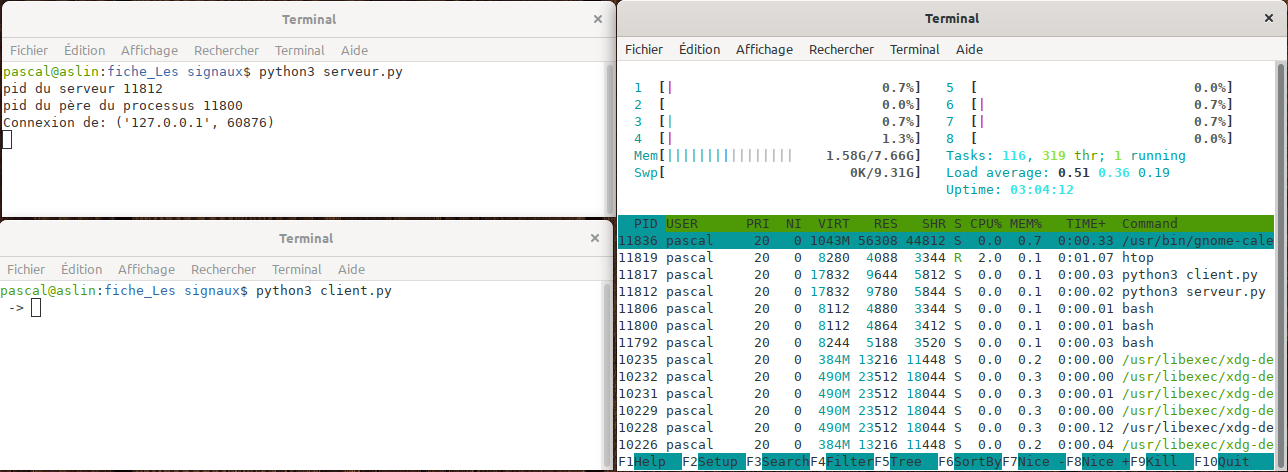
\includegraphics[width=1\linewidth]{bash_3x}

    
       \begin{enumerate}
           \item  Quel est le numéro pid du processus lié à  l'exécution de client.py ?
           
             \ifProf
                \textbf{La commande \textit{ htop}  nous indique que le pid du client.py est 11817.}
             \fi
           \item Quel(s) pourrait(aient) être le pid du parent du processus à  l'exécution de client.py ?
           
              \ifProf
           \textbf{Le parent est un programme \textit{bash}, donc en utilisant les informations de  \textit{htop} on voit qu'il peut s'agir du pid 11806 ou 11792}
           \fi
           \item Comment mettre fin au  processus associé serveur.py ? (donnez deux possibilités)
            
             \ifProf
           \textbf{En tapant Ctrl-C, avec  la fenêtre du terminal correspondant actif, en cliquant sur la croix de la fenêtre appropriée ou en tapant dans une console kill -2 11812.}
           \fi
       \end{enumerate}
        \item Tuez le serveur et continuez à envoyer des messages par le biais du client. Quelle message d'erreur apparaît? En expliquer la raison.
        Aurait-on pu procéder différemment ?
        
         \ifProf
        \textbf{On a l'erreur suivante : BrokenPipeError: [Errno 32] Broken pipe.\\ En fermant le serveur, le canal de communication n'est plus disponible rendant impossible l'écriture des données dans le PIPE (canal, tuyau). Le programme client a reçu un signal SIGPIPE.}
        
         \textbf{Il n'est pas nécessaire d'arrêter le serveur pour casser le canal de communication, on peut également exécuter la commande : } 
 kill -13 pid  (où pid est le numéro du processus à l'exécution du client).

        \fi
        
        \item Modifier le programme client pour que le programme prenne en considération cette erreur en demandant à l'utilisateur s'il veut continuer ou s'il veut mettre fin au programme.
        
        \ifProf
   
        \begin{code}{client.py}
            \inputminted[fontsize=\small]{Python}{client_cor.py}
        \end{code}
        \fi
    \end{enumerate}
    
\end{exercice}
\newpage
\section{Annexes}

\subsection{Description du fonctionnement CTRL-Z}

Dans le terminal 
% Nécessite le package tikz
\begin{center}
    \begin{tikzpicture}[
    f/.style={->,very thick,>=stealth'},%
    s/.style={draw,circle},%
    p/.style={fill=white,inner sep=3pt},scale=0.8]
    \node[fill=pink,inner sep=10pt] (T1) at (0,0) {shell} ;
    \node[s,fill=yellow] (Cat) at (-2,-3) {Proc 1} ;
   \draw(-2,-4)node{\footnotesize pid:5341};
    \node[s,fill=blue!8] (FG) at (3,-3) {Proc 2} ;
    \draw[f] (T1) -- (Cat) node[pos=0.5,p]{$cat$} ;
    \draw[dashed](-3,-2)rectangle(-1,-5)node(fg)[below]{travail de premier plan};
    \draw[dashed](2,-2)rectangle(4,-5)node[below]{travail d'arrière plan};
     \draw[f] (T1) -- (FG) node[pos=0.5,p]{$Cmd \&$} ;
     %\draw(4,-7)node[text width=5cm](sign){Les signaux Ctrl-C et Ctrl-Z s'adressent à ce(s)  travail(aux)};
     %\draw[->](sign.west) to [out=180,in=270](fg.south);
    \end{tikzpicture}
\end{center}
 La commande \textbf{Ctrl-Z } va passer le processus \textbf{cat} dans les travaux en arrière plan et changer son état en \textbf{Stopped} .  On aurait pu également taper la commande \textbf{kill SIGSTP 5341 } (\textit{si 5341 est le pid du processus de cat}). L'état \textbf{Stopped} du processus \textbf{cat}  interdit au processus de s'exécuter. La reprise est assurée à la réception du signal SIGCONT.
 
  \begin{center}
        \begin{tikzpicture}[
    f/.style={->,very thick,>=stealth'},%
    s/.style={draw,circle},%
    p/.style={fill=white,inner sep=3pt},scale=0.8]
    \node[fill=pink,inner sep=10pt] (T1) at (0,0) {shell} ;
    \node[s,fill=yellow] (Proc) at (-2,-2.7) {ps} ;
    \node[s,] (FG) at (5,-3) {Proc 2} ;
     \node[s,fill=blue!8] (Cat) at (3,-3) {Proc 1} ;
 \draw(3,-4)node{\footnotesize pid:5341};
    \node[s] (kill) at (-5,-1) {\small kill -2 5341} ;
   \draw[->](kill)--(-3,-3)node[midway,above,rotate=-45]{signal};
     
     \draw[f] (T1) to  (Proc) ;
    \draw[f] (T1) -- (Cat)  ;
     \draw[f] (T1) -- (FG) ;
    \draw[dashed](-3,-2)rectangle(-1,-5)node(fg)[below]{travail de premier plan};
    \draw[dashed](2,-2)rectangle(6,-5)node[below]{travail d'arrière plan};
    \draw(4,-7)node[text width=6.5cm](sign){Les signaux Ctrl-C et Ctrl-Z ne s'adressent qu'aux travaux de premier plan};
    \draw[->](sign.west) to [out=180,in=270](fg.south);

    \end{tikzpicture}
    
\end{center}
 La commande \textbf{killall -2 cat } n'a pas d'action sur le processus \textbf{cat}  car il ne fait partie des processus qui sont au premier plan. 
 
\noindent À l'aide de la commande \textbf{fg} (signal SIGCONT) le processus réintègre les processus de premier plan.

  \begin{center}
    \begin{tikzpicture}[
    f/.style={->,very thick,>=stealth'},%
    s/.style={draw,circle},%
    p/.style={fill=white,inner sep=3pt},scale=0.8]
    \node[fill=pink,inner sep=10pt] (T1) at (0,0) {shell} ;
   % \node[s,fill=yellow] (Proc) at (-2,-2.7) {ps} ;
    \node[s,fill=blue!8] (FG) at (3,-3) {Proc 2} ;
    \node[s,forbidden sign,fill=yellow] (Cat) at (-2,-3) {Proc 1} ;
    \draw(-2,-4)node{\footnotesize pid:5341};
    \node[s] (kill) at (-5,-1) {\small kill -2 5341} ;
    \draw[red, ->,very thick](kill) to (Cat) ;
    
   % \draw[f] (T1) to  (Proc) ;
    \draw[f] (T1) -- (Cat)  ;
    \draw[f] (T1) -- (FG) ;
    \draw[dashed](-3,-2)rectangle(-1,-5)node(fg)[below]{travail de premier plan};
    \draw[dashed](2,-2)rectangle(4,-5)node[below]{travail d'arrière plan};
    \draw(4,-7)node[text width=6cm](sign){Le signal SIGINT (kill -2) peut être délivré au processus destinataire, qui va se terminer, puisqu'il s'agit de l'action par défaut.};
    \draw[->](sign.west) to [out=180,in=270](fg.south);
    
    \end{tikzpicture}
    
    \end{center}


\newpage
\hypertarget{liste signaux}{%
\subsection{Signaux provoqués par une exception matérielle}\label{liste-signaux}}

source : \url{http://mat.free.free.fr/downloads/unix/signaux.pdf}
\begin{description}
    \item[SIGFPE]  Floating-point exception : envoyé lors d'un problème avec une opération en
    virgule flottante mais il est aussi utilisé pour l'erreur de division entière par
    zéro. L'action par défaut est la mise à mort du processus en créant un fichier
    d'image mémoire core. Ce fichier est alors utilisé par l'outil de "debugger"
    gdb.
    \item[SIGILL] Illegal instruction : envoyé au processus qui tente d'exécuter une instruction
    illégale. Ceci ne doit jamais se produire dans un programme normal mais il se
    peut que le fichier exécutable soit corrompu ( erreur lors du chargement en
    mémoire). L'action par défaut est la mise à mort du processus en créant un
    fichier d'image mémoire core.
    \item[SIGSEV] Segmentation violation : envoyé lors d'un adressage mémoire invalide (emploi
    d'un pointeur mal initialisé). L'action par défaut est la mise à mort du
    processus en créant un fichier d'image mémoire core.
    \item[SIGBUS] Bus error : envoyé lors d'une erreur d'alignement des adresses sur le bus.
    L'action par défaut est la mise à mort du processus en créant un fichier
    d'image mémoire core.
    \item[SIGTRAP] Trace trap : envoyé après chaque instruction, il est utilisé par les programmes
    de mise au point (debug).
    L'action par défaut est la mise à mort du processus en créant un fichier
\end{description}

\subsection{Signaux de terminaison ou d'interruption de processus}
\begin{description}
\item[SIGHUP] Hangup : envoyé à tous les processus attachés à un terminal lorsque celui-ci
est déconnecté du système. Il est courant d'envoyer le signal à certains
processus démons afin de leur demander de se réinitialiser. L'action par
défaut est la miseà mort du processus.
\item[SIGINT] Interrupt : le plus souvent déclenché par [Ctrl-C].
L'action par défaut est la mise à mort du processus.
\item[SIGQUIT] Quit : similaire à SIGINT mais pour [Ctrl-$\backslash$].
L'action par défaut est la mise à mort du processus en créant un fichier
d'image mémoire core.
\item[SIGIOT] I/O trap instruction : émis en cas de problème hardware (I/O). 
\item[SIGABRT] Abort : Arrêt immédiat du processus (erreur matérielle). à core
\item[SIGKILL] Kill : utilisé pour arrêter l'exécution d'un processus.
L'action par défaut est non modifiable.
\item[SIGTERM] Software termination : C'est le signal qui par défaut est envoyé par la
commande kill. L'action par défaut est la mise à mort du processus.
\end{description}

\subsection{Signaux utilisateurs}
\begin{description}
\item[SIGUSR1] User defined signal 1 : Définie par le programmeur. L'action par défaut est la
mise à mort du processus.
\item[SIGUSR2] User defined signal 2 : idem que SIGUSR1 .
\end{description}

\subsection{Signal généré pour un tube}
\begin{description}
    \item[SIGPIPE] Signal d'erreur d'écriture dans un tube sans processus lecteur.
    L'action par défaut est la mise à mort du processus.
\end{description}

\subsection{Signaux liés au contrôle d'activité}
\begin{description}
   \item[SIGCLD] Signal envoyé au processus parent lorsque les processus fils terminent.
Aucune action par défaut.
Signaux liés au contrôle d'activité
   \item[SIGCLD] Signal envoyé au processus parent lorsque les processus fils terminent.
Aucune action par défaut.
   \item[SIGCONT] L'action par défaut est de reprendre l'exécution du processus s'il est stoppé.
Aucune action si le processus n'est pas stoppé.
   \item[SIGSTOP] Suspension du processus.
L'action par défaut est la suspension ( !! non modifiable).
   \item[SIGTSTP] Emission à partir d'un terminal du signal de suspension [CTRL-Z]. Ce signal à
le même effet que SIGSTOP mais celui-ci peut être capturé ou ignoré.
L'action par défaut est la suspension.
   \item[SIGTTIN] Est émis par le terminal en direction d'un processus en arrière-plan qui essaie
de lire sur le terminal. L'action par défaut est la suspension.
   \item[SIGTTOU] Est émis par le terminal en direction d'un processus en arrière-plan qui essaie
d'écrire sur le terminal. L'action par défaut est la suspension.
\end{description}

\subsection{Signal lié à la gestion des alarmes}
\begin{description}
       \item[SIGALRM]
    Alarm clock : généré lors de la mise en route du système d'alarme par l'appel
    système alarm().
\end{description}

\newpage
\subsection*{Humour :  SIGTERM et SIGKILL \copyright Daniel Stori}
\begin{center}
    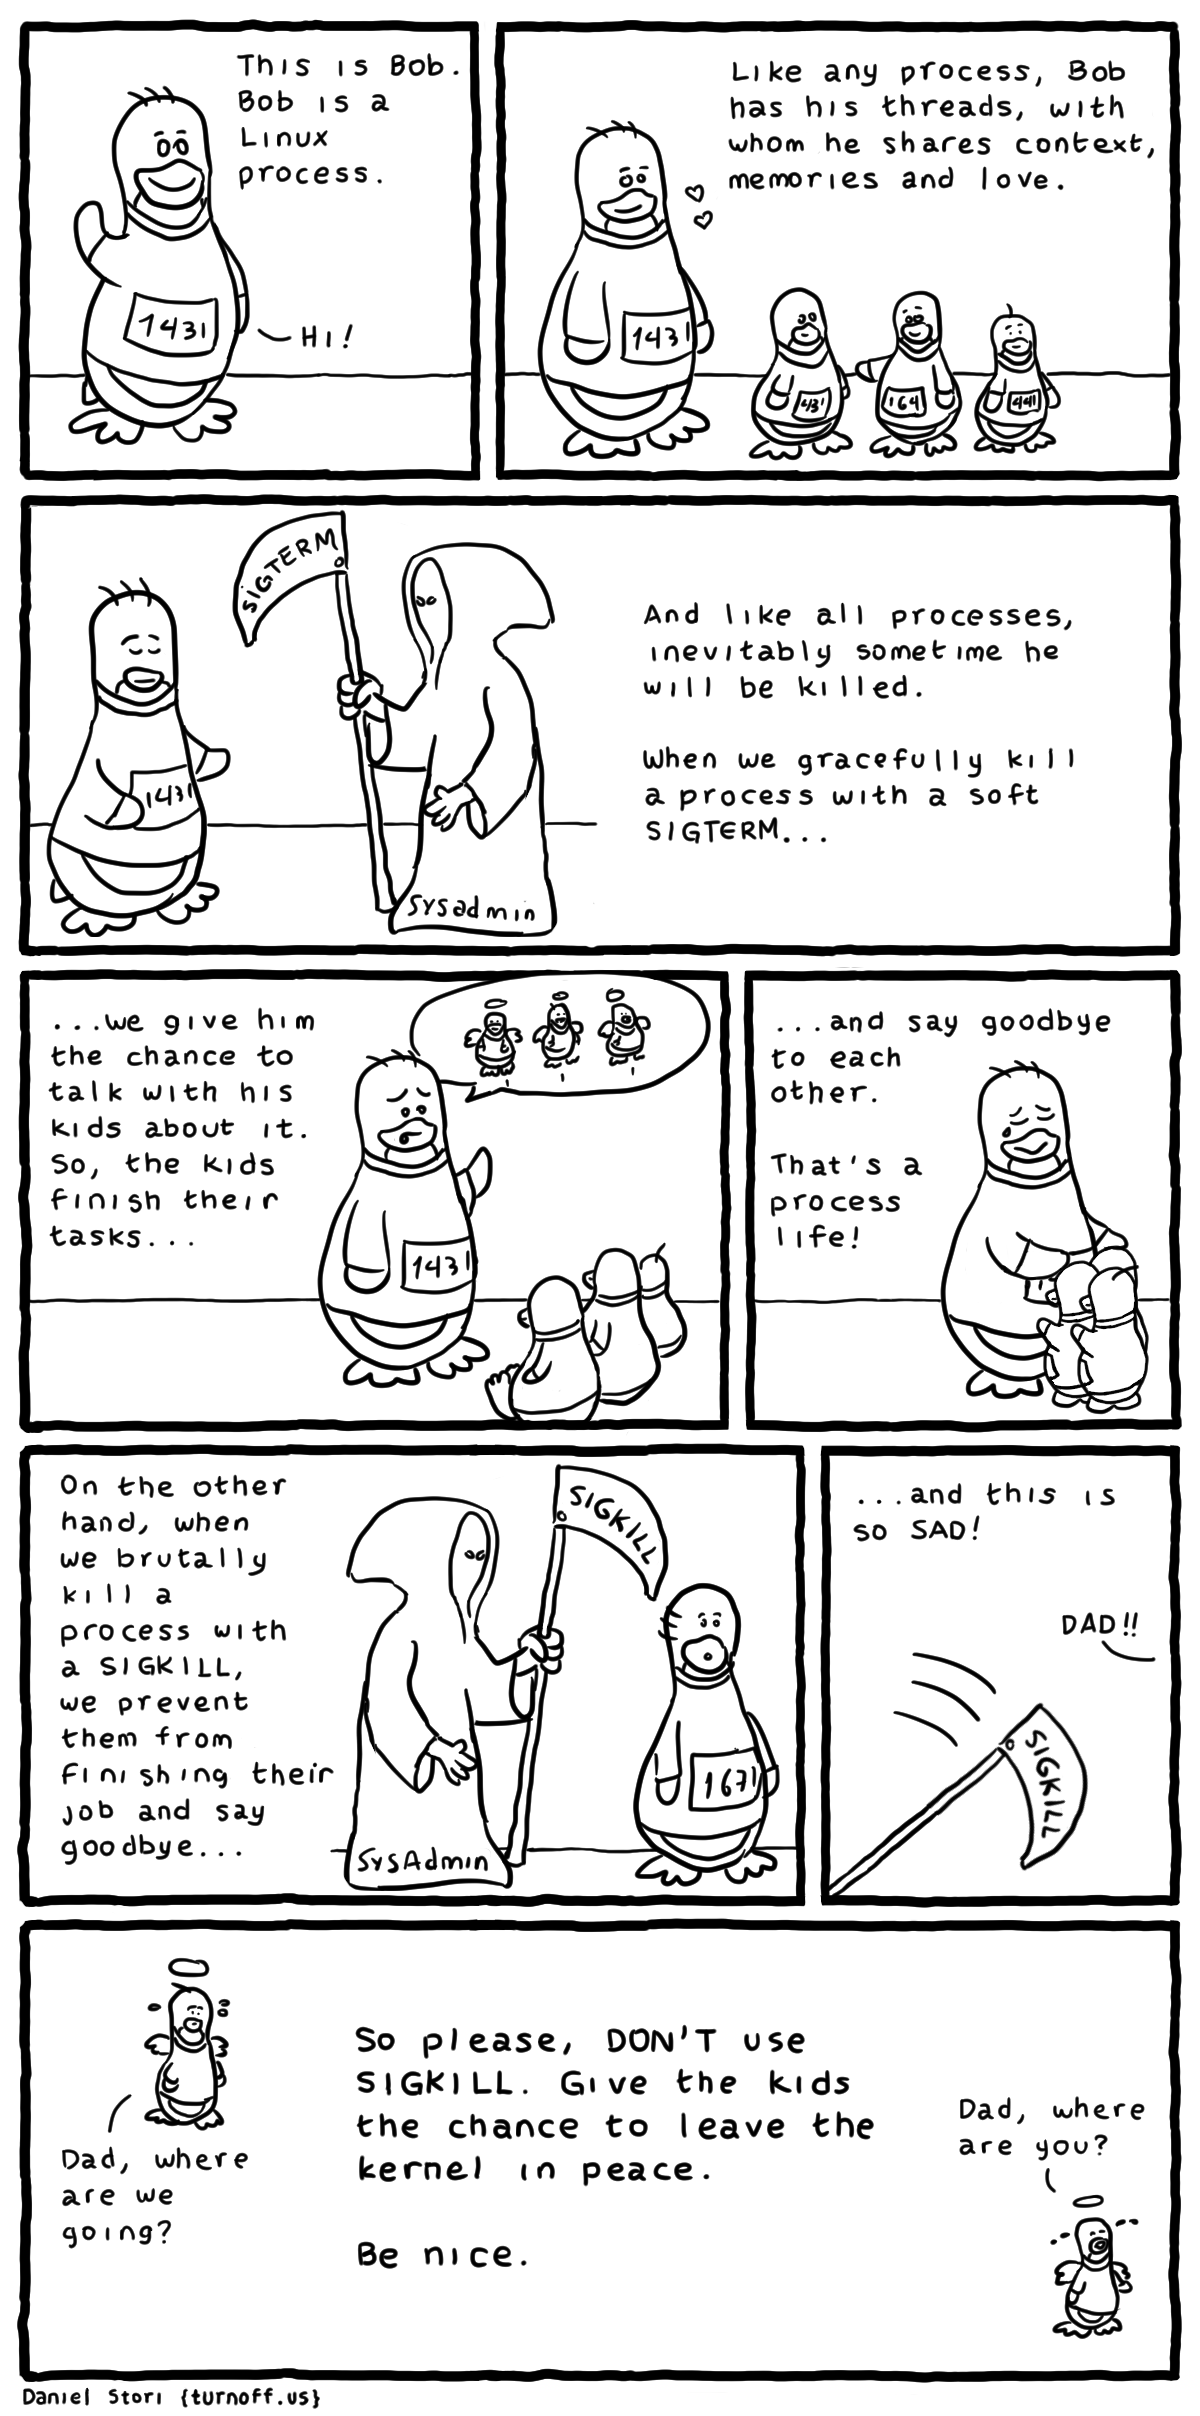
\includegraphics[width=0.75\linewidth]{dont-sigkill}
\end{center}

\end{document}
